\newcommand{\dpop}{\Delta p/p}

The initial goal of the spin coherence time (SCT) studies at COSY was to 
confirm the possibility of using sextupole fields in the correction of spin tune 
dispersion associated with the transverse beam emittances and 
momentum dispersion ($\dpop$).~\cite{COSY:SCT:IPAC15}
At the present moment, SCT optimization is the initial phase of any EDM-related 
investigation at COSY.

Sextupole spin decoherence suppression is used together with electron cooling, in order to minimize 
the beam's phase space volume, and bunching, which is used for the suppression of the linear spin
decoherence effect associated with momentum dispersion.
The sextupoles, placed in the arc sections, are used for the suppression of
second-order spin decoherence effects.

Spin decoherence is controlled by means of three sextupole families, marked respectively: MXG, 
placed in the maximum of the dispersion function, and controlling the decoherence associated with $\dpop$;
MXS, placed in the maximum of the horizontal beta-function $\beta_x$, and controlling the dispersion effect
associated with horizontal betatron oscilaltions; MXL, in the maximum of $\beta_y$, controlling the dispersion
assiciated with the vertical betatron oscillations.

\begin{figure}[h]\centering
	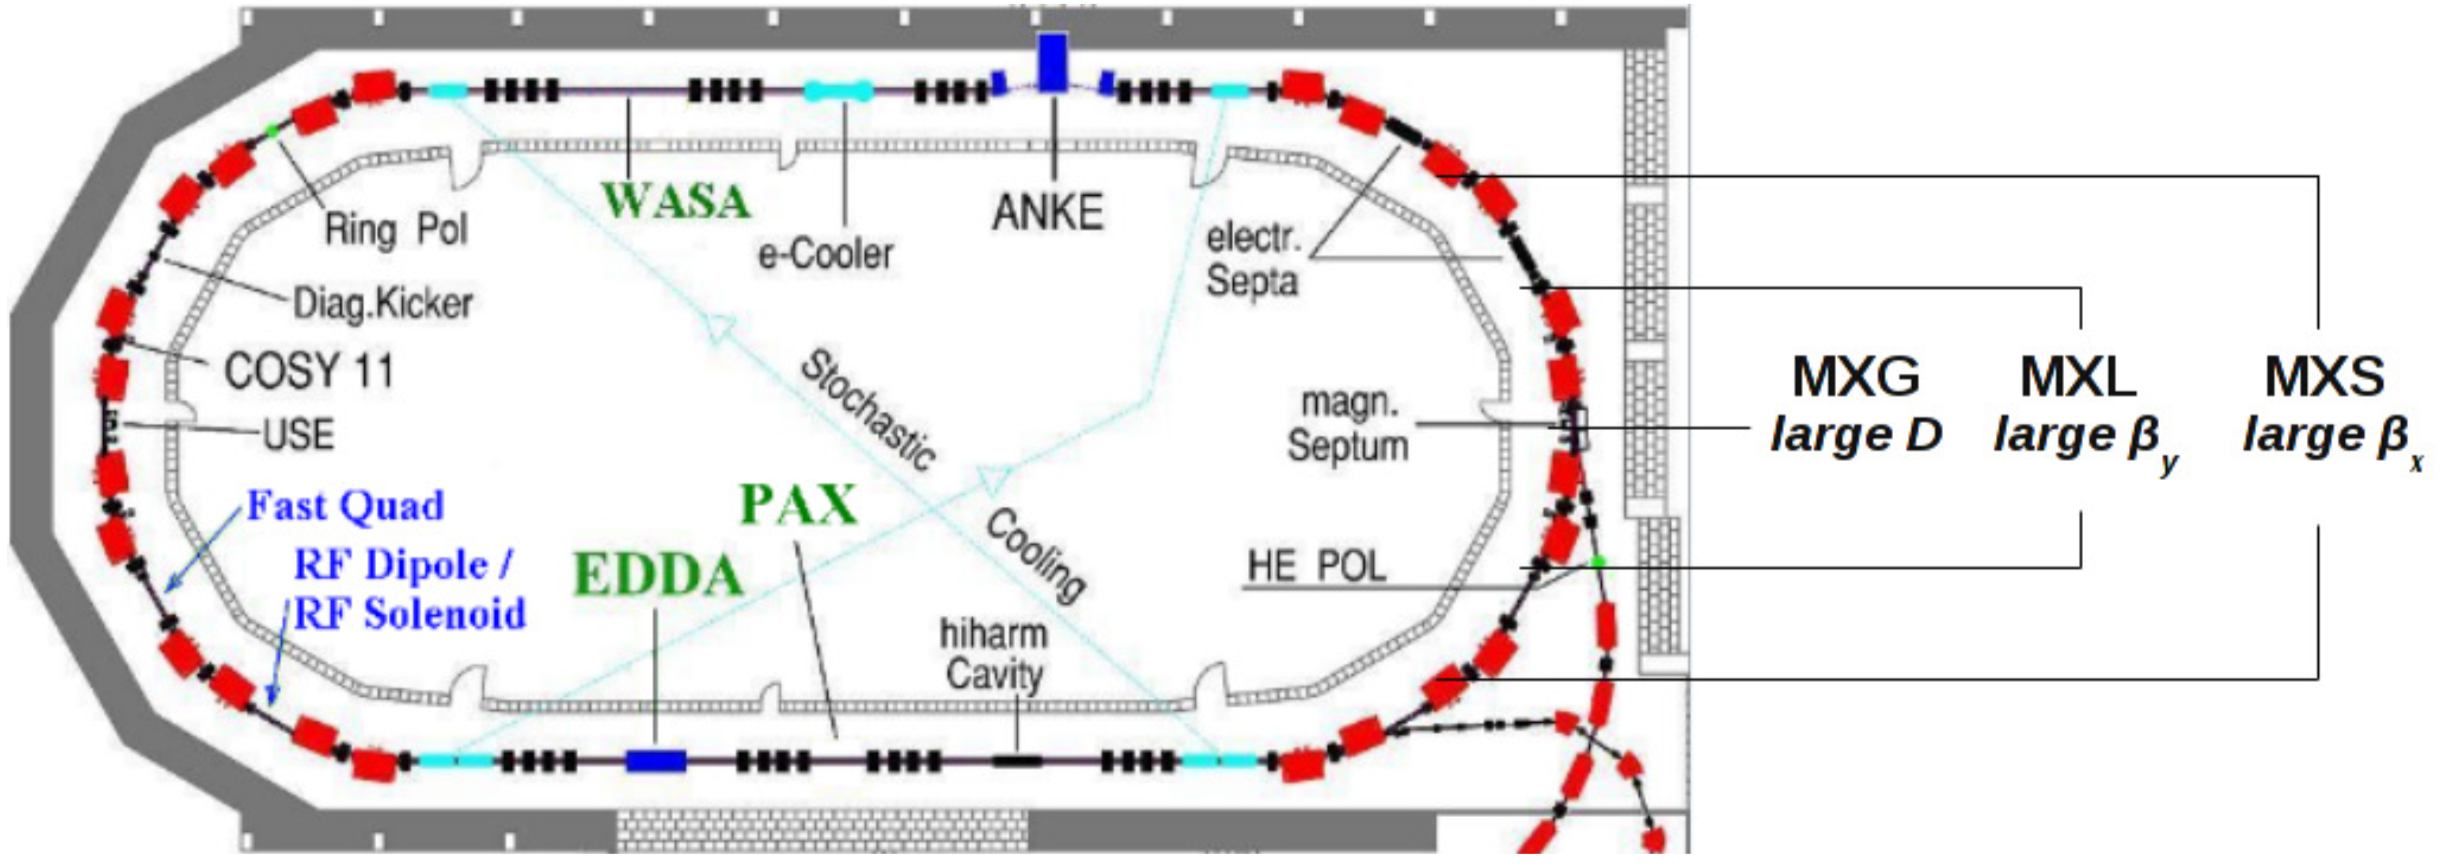
\includegraphics[width=\linewidth]{images/chapter4/COSY-sextupoles}
	\caption{COSY ring with marked sextupole positions. (Image taken from~\cite{Guidoboni:STORI14}.)}
\end{figure}

\subsection{Optimization procedure}
In this section we describe the optimization procedure using the example of the 2014 experiment.~\cite{Guidoboni:STORI14}
The SCT optimization experiment was first performed in 2012, but then only the MXS field strength was varied.
In 2014, a comprehensive (the field strengths of all three sextupole families were varied) SCT optimization
study was done for the first time.

To separate the effects related to the beam emittances and the 
second-order momentum dispersion $(\dpop)^2$, the beam was prepared in two different ways.

When studying the effect associated with a large $(\dpop)^2$, a polarized deuteron beam injected 
at $p=0.97$~GeV/c momentum is first cooled for 60 seconds, so that its emittance is minimized. 
After the cooling is turned off, the beam is bunched (harmonic number $h=1$). 
Bunching is required to minimize linear spin decoherence effects.

When studying the effect associated with horizontal emittance,~\footnote{Decoherence associated with 
	vertical emittance could not be studied because of acceptance limitations.} the beam is 
cooled and bunched simultaneously for the initial 60 seconds, after which cooling is turned off,
and horizontal heating is turned on for 5 seconds. The beam is heated by applying white noise to 
the horizontal kicker plates.

In both cases the polarization is vertically-oriented at injection. It is flipped by an RF solenoid 
after the beam preparation at the 80-th second.

Polarization is continuously measured by extracting the beam onto a 17 mm thick carbon target and
detecting the scattered deuterons at the EDDA polarimeter. 
Extraction is done by applying white noise to the vertical kicker. Elastic scattering of deuterons on 
carbon is a spin sensitive process with a large cross section.

The EDDA scintillators were grouped in four sectors (up, right, down, left); event rate asymmetry between the
left and right sectors is proportional to the beam's vertical polarization, the one between the up and down -- 
to the horizontal polarization component. Horizontal plane spin precession occurs at a a rate which greatly exceeds the polarimeter sampling rate, which is why a special data acquisition system was developed in 2012.~\cite{COSY:DAQ}

As a result of the experiment~\cite{Guidoboni:STORI14} a possibility of reaching an SCT over 1,000 seconds at COSY was shown. 

\subsection{SCT change when going from the external to the internal beam layers}
SCT optimization results obtained during the April-May 2019 beam time are shown below.

In the Figure series~\ref{fig:April2019:Polarization} the up-down cross section asymmetry measurement 
results are presented. In the first two figures one can observe that the rate of depolarization changes from
high in the first half (100 to 150 seconds) of the measurement cycle to significantly lower in the second half.
In Figure~\ref{fig:Polariation:recovery-from-halo-to-core} especially, we observe that polarization is increasing in the 130 to 150 second range, before it begins to gradually decrease again.
\begin{figure}[h]\centering
	\begin{subfigure}{\linewidth}
		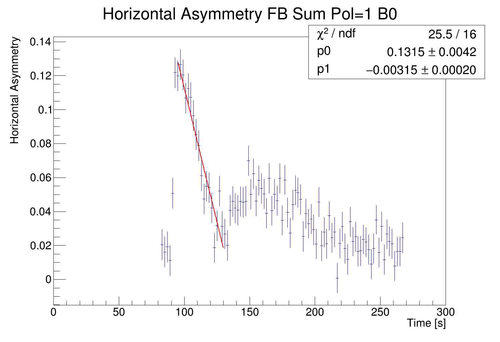
\includegraphics[height=.35\paperheight]{images/chapter4/SCT-April-2019/11th_19-55}
		\caption{SCT = $20.87 \pm 1.49$ sec.\label{fig:Polariation:recovery-from-halo-to-core}}
	\end{subfigure}
	\begin{subfigure}{\linewidth}
		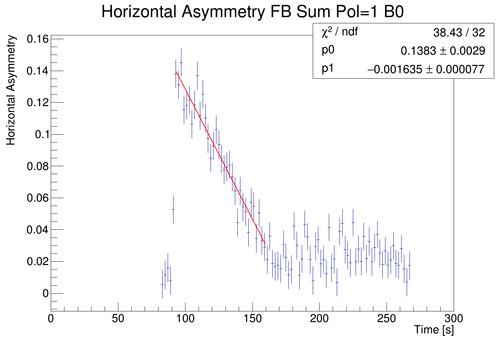
\includegraphics[height=.35\paperheight]{images/chapter4/SCT-April-2019/11th_20-20}
		\caption{SCT = $42.3 \pm 2.2$ sec.}
	\end{subfigure}
\end{figure}
\begin{figure}[h]\ContinuedFloat\centering
	\begin{subfigure}{\linewidth}
		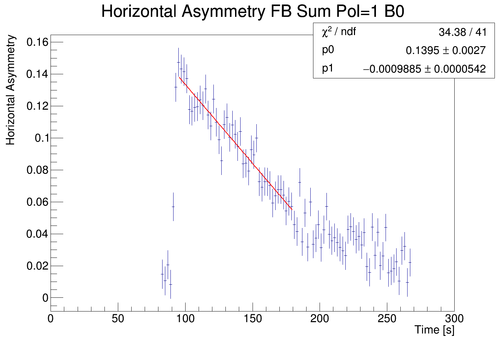
\includegraphics[height=.35\paperheight]{images/chapter4/SCT-April-2019/11th_20-31}
		\caption{SCT = $70.6 \pm 4.1$ sec.\label{fig:Polarization:halo-and-core-similar}}
	\end{subfigure}
	\begin{subfigure}{\linewidth}
		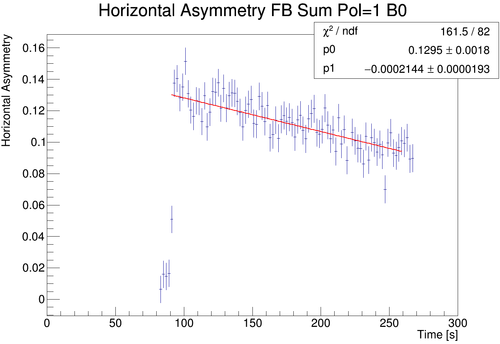
\includegraphics[height=.35\paperheight]{images/chapter4/SCT-April-2019/13th_03-23}
		\caption{SCT = $302.0 \pm 27.5$ sec.}
	\end{subfigure}
	\caption{Horizontal polarization measurements during SCT optimization during the axion search experiment done in April-May 2019.\label{fig:April2019:Polarization}}
\end{figure}

Such behavior can be explained by the non-uniformity of the polarization distribution. In the first half
of the measurement cycle particles from the outer (halo) beam layer are being sampled, while by the second half
those get exhausted, and the polarization of the internal (core) layer is being probed. Since the core is
more dense than the halo, the orbit length (hence spin tune) dispersion is less pronounced 
for its particles.

\subsection{SCT dependence on sextupole strength}
SCT dependence on the relative strengths of, respectively, the 
MXL and MXG sextupoles, measured during the April-May 2019 beamtime
is presented in Figure~\ref{fig:SCT_scan}. A resonance-type pattern can be observed.

\begin{figure}[h]\centering
	\begin{subfigure}{\linewidth}
		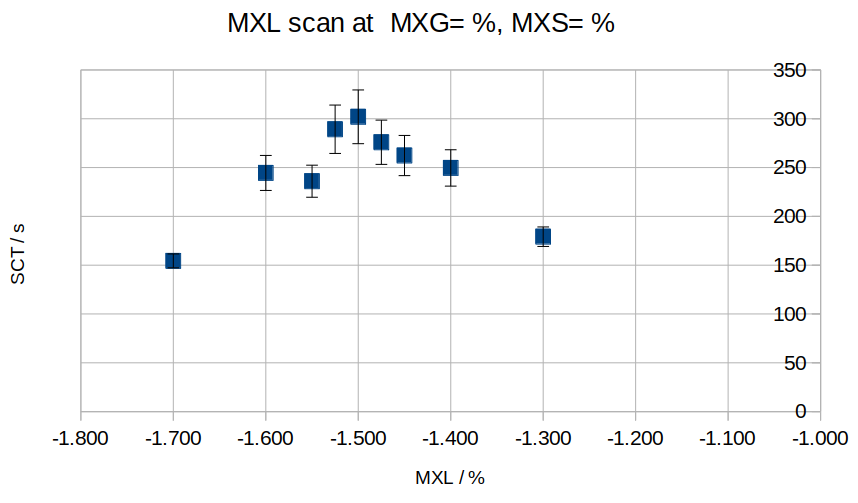
\includegraphics[height=.35\paperheight]{images/chapter4/SCT-April-2019/MXL_scan}
		\caption{MXL sextupole.}
	\end{subfigure}
	\begin{subfigure}{\linewidth}
		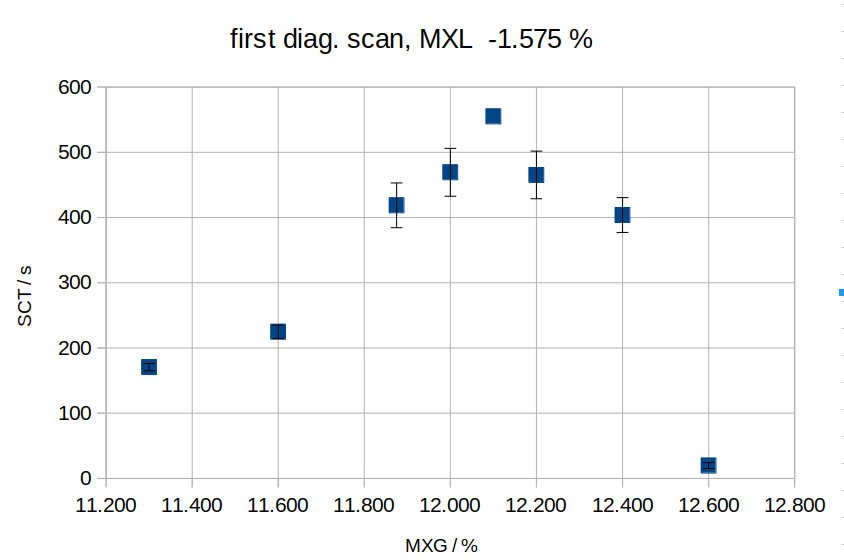
\includegraphics[width=.6\paperheight]{images/chapter4/SCT-April-2019/MXG_scan}
		\caption{MXG sextupole}
	\end{subfigure}
	\caption{SCT as a function fo the sextupole strength.\label{fig:SCT_scan}}
\end{figure}

Since COSY operates at an energy that is significantly far removed from spin resonance 
we decided to check if this pattern can be seen (within the framework of our numerical model) 
in the FS-type lattice. 
Spin tune standard deviation as a function of the corresponding sextupole gradient is plotted in Figure~\ref{fig:SCT_resonance}. 
(Data were taken from the simulation described in section~\ref{sec:decoh:sim-imperfect}.)
The same resonance pattern is observed as in the experiment.

\begin{figure}[h]
	\centering
	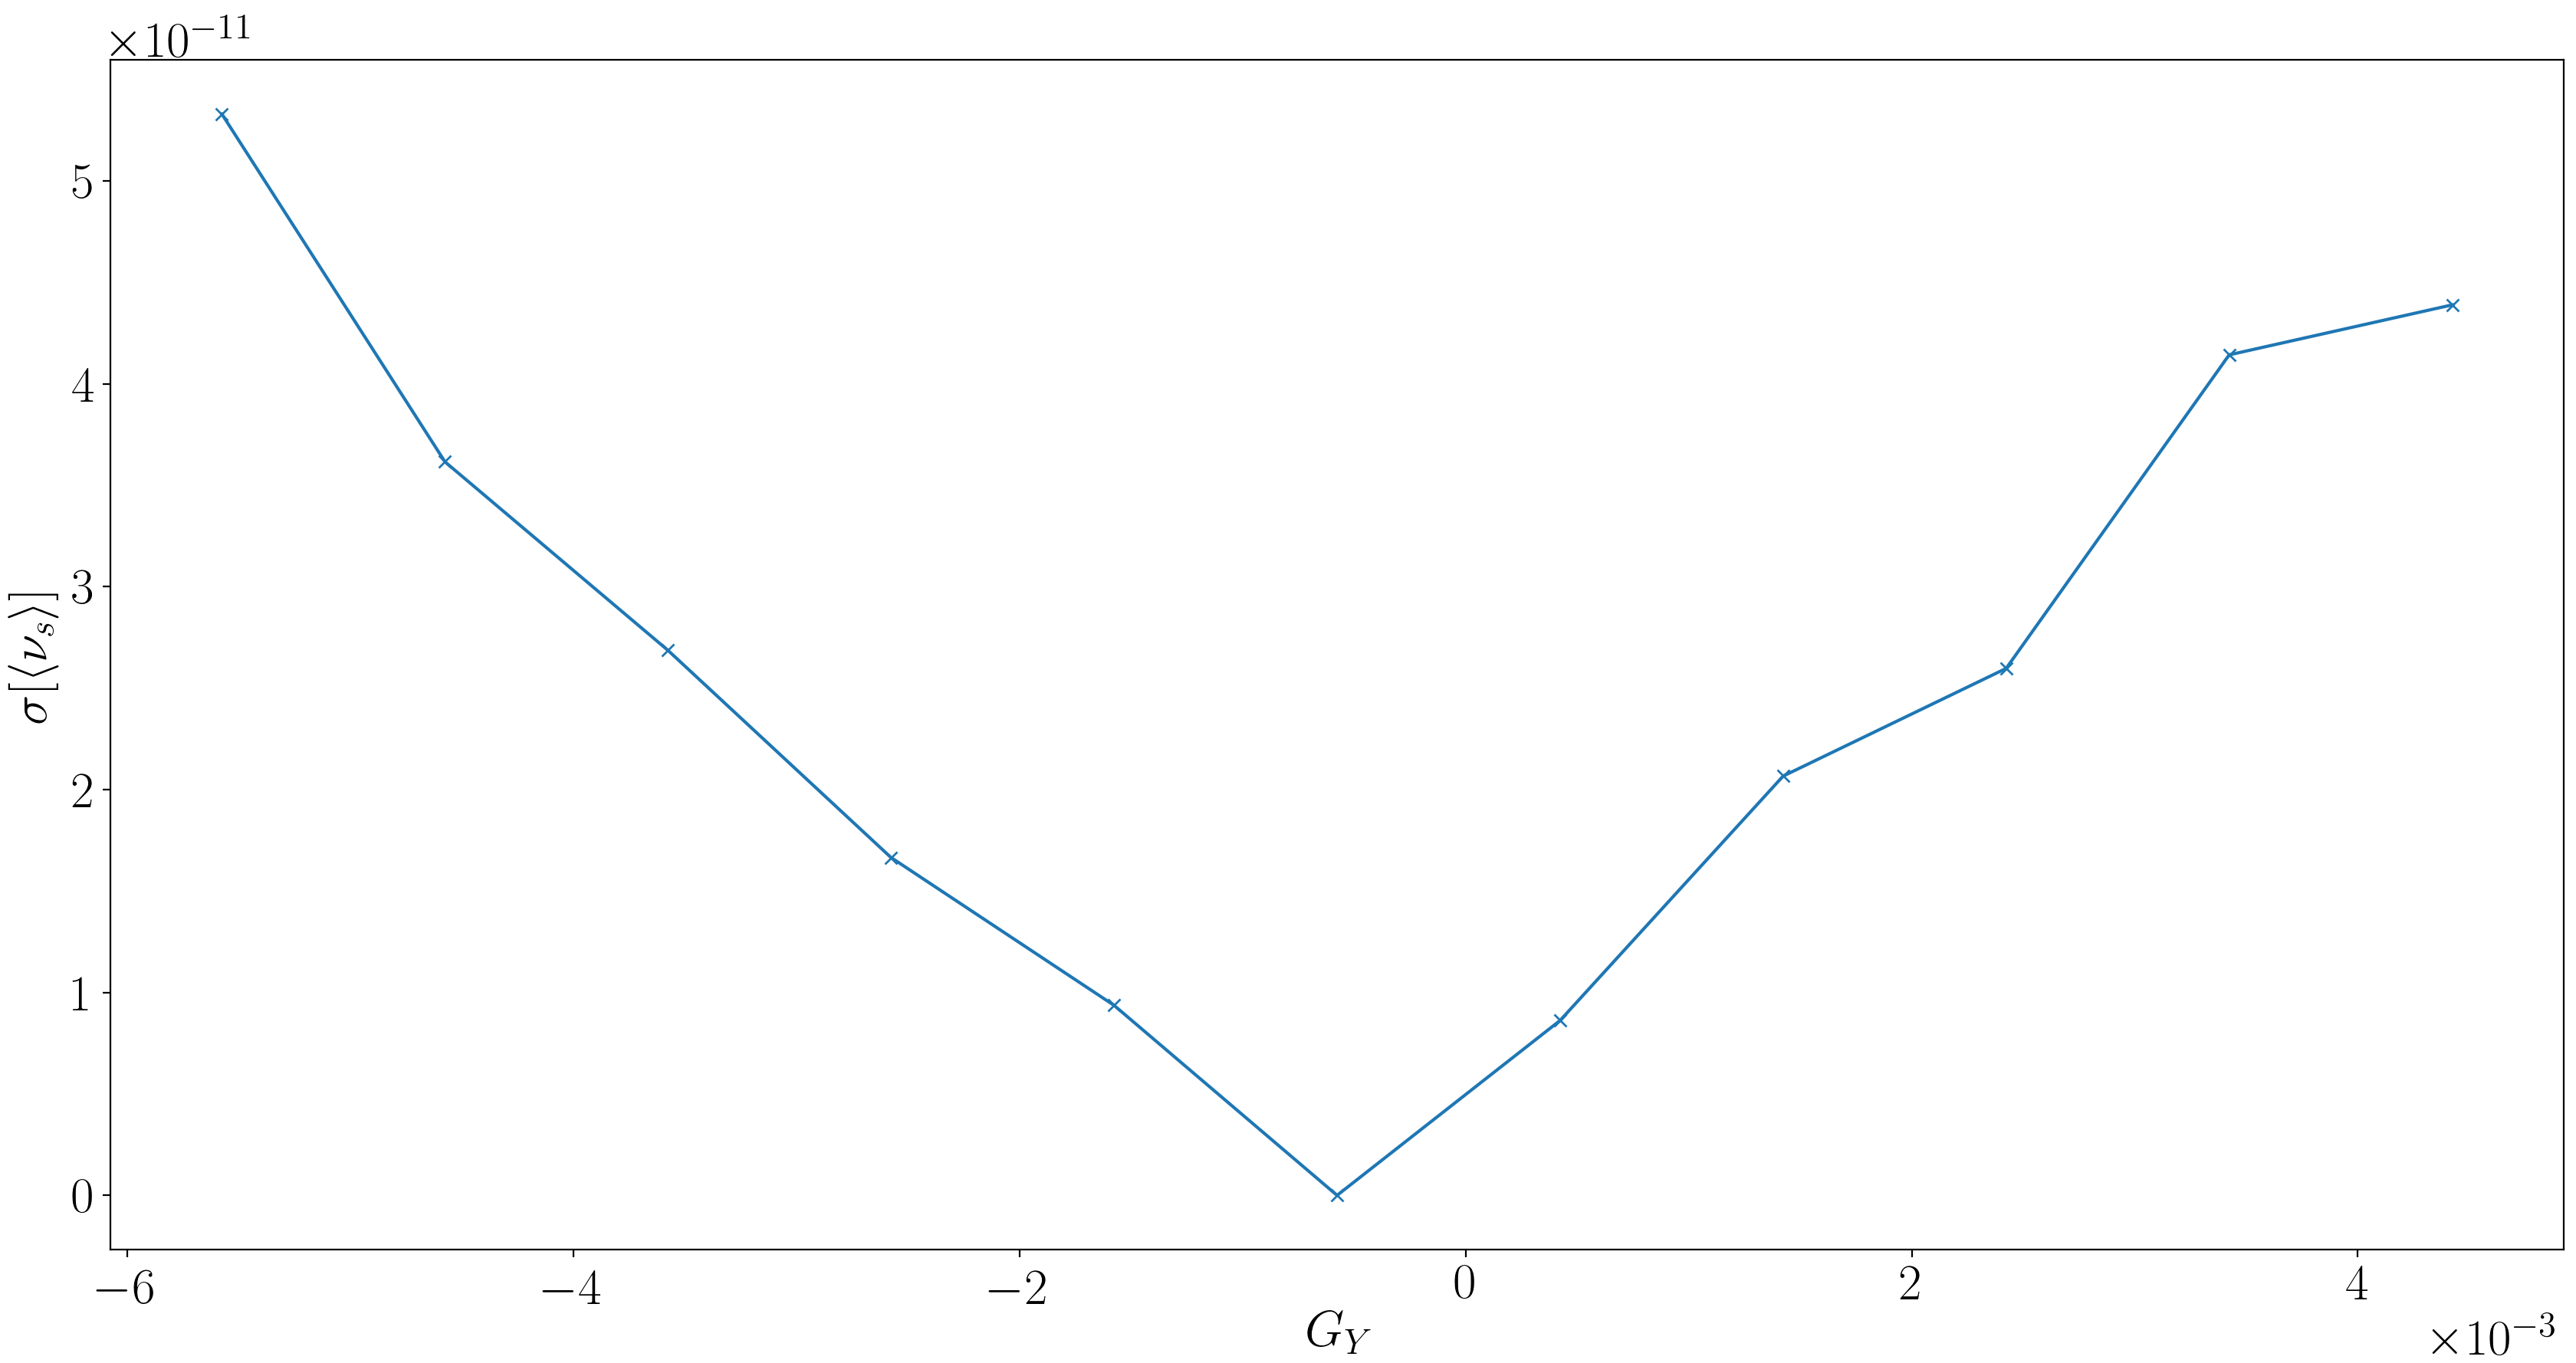
\includegraphics[width=\linewidth]{images/decoh_sim/stune_sd_vs_sext_strength_resonance}
	\caption{Spin tune dispersion as a function of the sextupole field gradient.\label{fig:SCT_resonance}}
\end{figure}
